\documentclass[12pt,letterpaper]{article}
\usepackage[utf8]{inputenc}
\usepackage{float, xcolor}

%----- Configuración del estilo del documento------%
\usepackage{graphicx, fancyhdr, lastpage}
\usepackage{enumitem, pifont}
\usepackage[left=2cm,right=2cm,top=1.8cm,bottom=2.3cm]{geometry}

%------ Paquetes matemáticos básicos --------%
\usepackage{amsmath, amssymb, amsthm}

\newcommand{\imp}{\rightarrow}
\newcommand{\vp}{\varphi}

\begin{document}

%------ Encabezado -------- %
\hrule height 0.1pt
\bigskip

\begin{center}
  \begin{minipage}{3cm}
    \begin{center}
      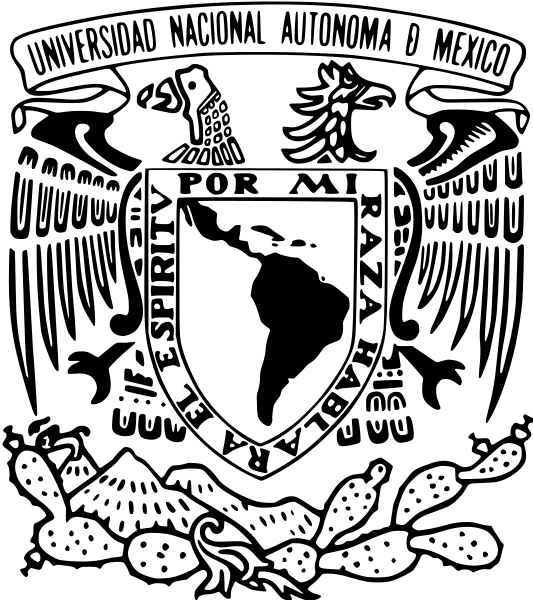
\includegraphics[height=3.4cm]{../unam_logo.png}
    \end{center}
  \end{minipage}\hfill
  \begin{minipage}{10cm}
    \begin{center}
      \textbf{\Large Universidad Nacional Autónoma de México}\\[0.2cm]
      \textbf{\large Facultad de Ciencias}\\[0.2cm]
      \textbf{Lógica Computacional | 2025-2}\\[0.4cm]
      \textbf{\Large Tarea 04}\\[0.1cm]
      \textbf{Docentes:}\\
      Noé Hernández \hspace{0.9em} Santiago Escamilla \hspace{0.9em} Ricardo López\\[0.3cm]
      \textbf{Autores:}\\
      Fernanda Ramírez Juárez \quad Ianluck Rojo Peña\\[0.3cm]
      \textbf{Fecha de entrega:} Martes 1 de abril de 2025
    \end{center}
  \end{minipage}\hfill
  \begin{minipage}{3cm}
    \begin{center}
      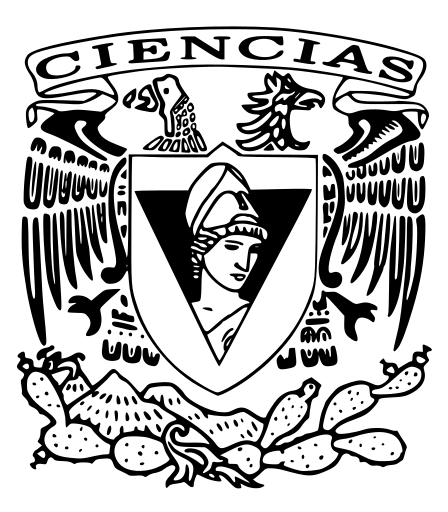
\includegraphics[height=3.4cm]{../fc_logo.png}
    \end{center}
  \end{minipage}
\end{center}

\bigskip
\hrule height 0.1pt
\bigskip

%------ Notas sobre la resolución --------%
\section*{Notas sobre la resolución.}

\begin{quote}
  \textbf{Nota general:} Cada ejercicio fue resuelto en base, y tomando como referencia, las notas de clase lcNota9.pdf, lcNota10.pdf, y lcNota11.pdf.
  
  Adem\'{a}s de las clases presenciales impartidas por el profesor y ayudantes, tanto para resolver dudas como las pistas y consejos dados
\end{quote}

\bigskip
\hrule height 0.1pt
\bigskip

\newpage
%------ Contenido -------- %
\section*{Resolución de Ejercicios.}

\begin{enumerate}
\item (1.5 pts.) Muestre mediante tableaux semánticos que
  \[
  \left\{ 
  \forall x \forall y \forall z (R(x,y) \wedge R(y,z) \rightarrow R(x,z)),
  \forall x \forall y (R(x,y) \rightarrow R(y,x)),
  \forall x \exists y R(x,y) 
  \right\} 
  \vDash \forall x R(x,x)
  \]
  % -- Respuesta --
  \begin{center}
    \hspace{-1.2cm} 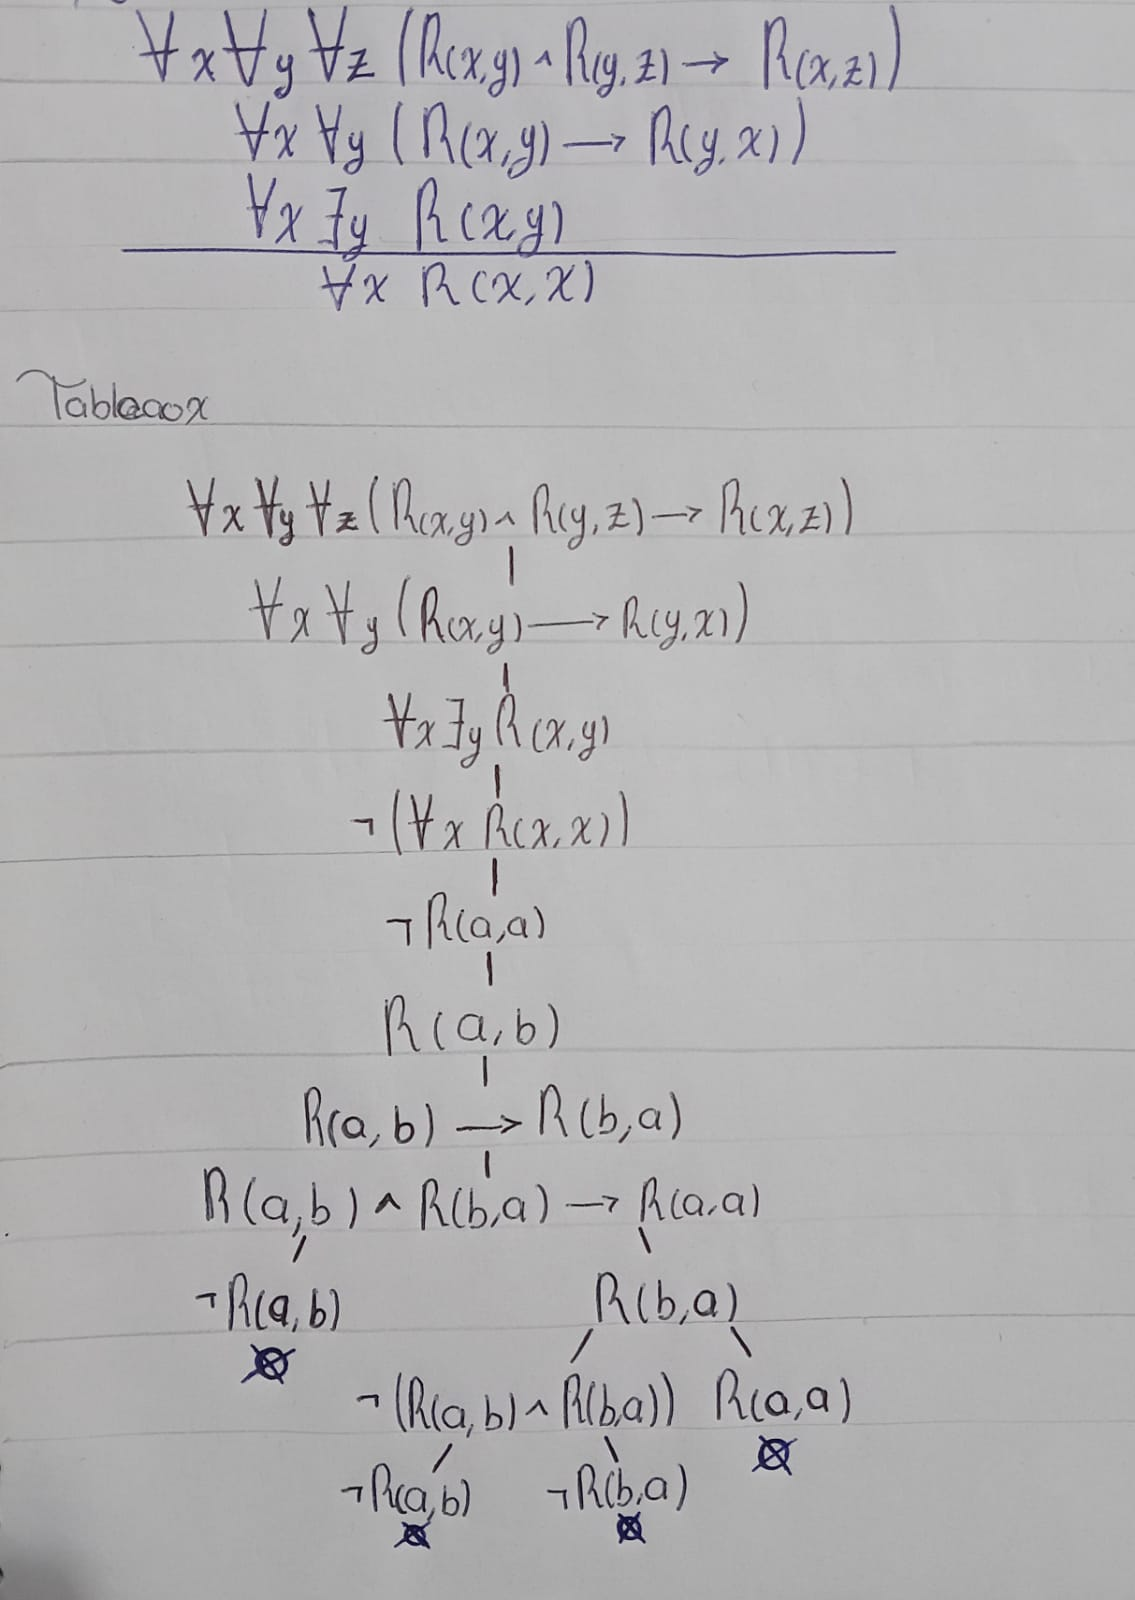
\includegraphics[width=\textwidth,height=0.8\textheight,keepaspectratio]{ejercicio1.png}
  \end{center}

  \[
  \hspace{-1cm}\therefore \text{ Se cumple } \forall \text{$x R(x,x)$}
  \]
  
  \newpage
  
\item (2 pts.) Transforme cada una de las siguientes fórmulas en forma normal clausular. Escriba cada uno de los pasos que utilizó.
  \begin{itemize}
  \item \( \forall x \forall y (\exists z P(z) \wedge \exists u (Q(x,u) \rightarrow \exists v Q(y,v))) \)
  \item \( \forall x \forall y \left( Q(x,y) \leftrightarrow \forall z (P(z,x) \leftrightarrow P(z,y)) \right) \)
  \end{itemize}
  
  % -- Respuesta --

  Utilizamos el Algoritmo de Skolem para transformar cada f\'{o}rmula en su forma clausular:\\
  
  \textbf{Input:} \( \forall x \forall y \Big(\exists z P(z) \wedge \exists u \big(Q(x,u) \rightarrow \exists v Q(y,v)\big)\Big) \)

  $(L)$ Limpiamos la f\'{o}rmula: \checkmark

  \quad \ding{228} $\forall x \forall y \Big(\exists z P(z) \wedge \exists u \big(Q(x,u) \rightarrow \exists v Q(y,v)\big)\Big)$
  \\
  
  $(I)$ Eliminamos las implicaciones y bi-condicionales empleando las equivalencias, para este caso tenemos:
  \[
    Q(x, y) \imp \exists v Q(y, v) \equiv \neg Q(x, y) \lor \exists v Q(y, v)
  \]

  \quad \ding{228} $\forall x \forall y \Big(\exists z P(z) \wedge \exists u \big(\neg Q(x, y) \lor \exists v Q(y, v)\big)\Big)$
  \\

  $(N)$ Manipulamos la negaci\'{o}n para permitir su efecto \'{u}nicamente en f\'{o}rmulas at\'{o}micas adem\'{a}s de quitar las doble negaciones: \checkmark

  \quad \ding{228} $\forall x \forall y \Big(\exists z P(z) \wedge \exists u \big(\neg Q(x, y) \lor \exists v Q(y, v)\big)\Big)$
  \\
  
  $(R)$ Renombramos variables ligadas para que ninguna variable se repita en los cuantificadores: \checkmark

  \quad \ding{228} $\forall x \forall y \Big(\exists z P(z) \wedge \exists u \big(\neg Q(x, y) \lor \exists v Q(y, v)\big)\Big)$
  \\

  $(E)$ Extraemos cuantificadores de la matriz:

  \quad \ding{228} $\forall x \forall y \exists z \exists u \exists v \Big(P(z) \wedge \big(\neg Q(x, y) \lor Q(y, v)\big)\Big)$
  \\

  $(D)$ Usamos las leyes distributivas para transformar la matriz a FNC. La f\'{o}rmula est\'{a} ahora en FNCP: \checkmark

  \quad \ding{228} $\forall x \forall y \exists z \exists u \exists v \Big(P(z) \wedge \big(\neg Q(x, y) \lor Q(y, v)\big)\Big)$
  \\
  
  $(S)$ Recorremos el prefijo de izquierda a derecha y aplicamos las respectivas \textit{funciones de Skolem}:
  
  \quad \ding{228} $\forall x \forall y \bigg(P\big(f(x, y) \big) \land \Big(\neg Q\big(x,\; h(x, y)\big) \lor Q\big(y,\; g(x, y)\big)\Big)\bigg)$

  \[
  \therefore \text{La Forma Normal Clausular de la f\'{o}rmula es:}
  \]

  \begin{center}
    \textbf{Output:} $\big\{\: \{P\big(f(x, y)\big)\},\; \{\neg Q\big(x,\; h(x, y)\big),\; Q\big(y,\; g(x, y)\big) \}\: \big\}$
  \end{center}

  \newpage
  
  \textbf{Input:} \( \forall x \forall y \Big( Q(x,y) \leftrightarrow \forall z \big(P(z,x) \leftrightarrow P(z,y)\big) \Big) \)

  $(L)$ Limpiamos la f\'{o}rmula: \checkmark

  \quad \ding{228} $\forall x \forall y \Big( Q(x,y) \leftrightarrow \forall z \big(P(z,x) \leftrightarrow P(z,y)\big) \Big)$
  \\
  
  $(I)$ Eliminamos las implicaciones y bi-condicionales empleando las equivalencias, para este caso tenemos:
  \[
  P(z,x) \leftrightarrow P(z,y) \equiv \big(\neg P(z,x) \lor P(z,y) \big) \land \big(P(z,x) \lor \neg P(z,y) \big)
  \]

  \quad \ding{228} $\forall x \forall y \bigg( Q(x,y) \leftrightarrow \forall z \Big( \big(\neg P(z,x) \lor P(z,y) \big) \land \big(P(z,x) \lor \neg P(z,y) \big) \Big) \bigg)$

  \[
  Q(x,y) \leftrightarrow \forall z \Big( \big(\neg P(z,x) \lor P(z,y) \big) \land \big(P(z,x) \lor \neg P(z,y) \big) \Big)
  \]
  \[
  \equiv
  \]
  \[
  \bigg(\neg Q(x,y) \: \lor \: \forall z \Big( \big(\neg P(z,x) \lor P(z,y) \big) \land \big(P(z,x) \lor \neg P(z,y) \big) \Big)\bigg)
  \]
  \[
  \land
  \]
  \[
  \bigg( Q(x,y) \: \lor \: \neg \forall z \Big( \big(\neg P(z,x) \lor P(z,y) \big) \land \big(P(z,x) \lor \neg P(z,y) \big) \Big) \bigg)
  \]

  \quad \ding{228} $\forall x \forall y \Bigg (\bigg(\neg Q(x,y) \: \lor \: \forall z \Big( \big(\neg P(z,x) \lor P(z,y) \big) \land \big(P(z,x) \lor \neg P(z,y) \big) \Big)\bigg)$

  \hspace{2cm} $\land \bigg( Q(x,y) \: \lor \: \neg \forall z \Big( \big(\neg P(z,x) \lor P(z,y) \big) \land \big(P(z,x) \lor \neg P(z,y) \big) \Big) \bigg)\Bigg)$
  \\

  $(N)$ Manipulamos la negaci\'{o}n para permitir su efecto \'{u}nicamente en f\'{o}rmulas at\'{o}micas adem\'{a}s de quitar las doble negaciones:

  \[
  \bigg( Q(x,y) \: \lor \: \neg \forall z \Big( \big(\neg P(z,x) \lor P(z,y) \big) \land \big(P(z,x) \lor \neg P(z,y) \big) \Big) \bigg)\Bigg)
  \]
  \[
  \equiv
  \]
  \[
  \bigg( Q(x,y) \: \lor \: \exists z \neg \Big( \big(\neg P(z,x) \lor P(z,y) \big) \land \big(P(z,x) \lor \neg P(z,y) \big) \Big) \bigg)
  \]
  \[
  \equiv
  \]
  \[
  \bigg( Q(x,y) \: \lor \: \exists z \Big( \neg \big(\neg P(z,x) \lor P(z,y) \big) \lor \neg \big(P(z,x) \lor \neg P(z,y) \big) \Big) \bigg)
  \]
  \[
  \equiv
  \]
  \[
  \bigg( Q(x,y) \: \lor \: \exists z \Big( \big(P(z,x) \land \neg P(z,y) \big) \lor \big(\neg P(z,x) \land P(z,y) \big) \Big) \bigg)
  \]

  \quad \ding{228} $\forall x \forall y \Bigg (\bigg(\neg Q(x,y) \: \lor \: \forall z \Big( \big(\neg P(z,x) \lor P(z,y) \big) \land \big(P(z,x) \lor \neg P(z,y) \big) \Big)\bigg)$

  \hspace{2cm} $\land \bigg( Q(x,y) \: \lor \: \exists z \Big( \big(P(z,x) \land \neg P(z,y) \big) \lor \big(\neg P(z,x) \land P(z,y) \big) \Big) \bigg)\Bigg)$
  \\
  
  $(R)$ Renombramos variables ligadas para que ninguna variable se repita en los cuantificadores:

  \quad \ding{228} $\forall x \forall y \Bigg (\bigg(\neg Q(x,y) \: \lor \: \forall z \Big( \big(\neg P(z,x) \lor P(z,y) \big) \land \big(P(z,x) \lor \neg P(z,y) \big) \Big)\bigg)$

  \hspace{2cm} $\land \bigg( Q(x,y) \: \lor \: \exists w \Big( \big(P(w,x) \land \neg P(w,y) \big) \lor \big(\neg P(w,x) \land P(w,y) \big) \Big) \bigg)\Bigg)$
  \\

  $(E)$ Extraemos cuantificadores de la matriz:

  \quad \ding{228} $\forall x \forall y \forall z \exists w \Bigg (\bigg(\neg Q(x,y) \: \lor \: \Big( \big(\neg P(z,x) \lor P(z,y) \big) \land \big(P(z,x) \lor \neg P(z,y) \big) \Big)\bigg)$

  \hspace{3cm} $\land \bigg( Q(x,y) \: \lor \: \Big( \big(P(w,x) \land \neg P(w,y) \big) \lor \big(\neg P(w,x) \land P(w,y) \big) \Big) \bigg)\Bigg)$
  \\

  $(D)$ Usamos las leyes distributivas para transformar la matriz a FNC. La f\'{o}rmula est\'{a} ahora en FNCP: \checkmark
  \[
  (1)\; \neg Q(x,y) \: \lor \: \Big( \big(\neg P(z,x) \lor P(z,y) \big) \land \big(P(z,x) \lor \neg P(z,y) \big) \Big)
  \]
  \[
  \equiv
  \]
  \[
  (1)\; \big(\neg Q(x,y) \lor \neg P(z,x) \lor P(z,y) \big) \land \big(\neg Q(x,y) \lor P(z,x) \lor \neg P(z,y) \big)
  \]
  
  \[
  (2)\; Q(x,y) \: \lor \: \Big( \big(P(w,x) \land \neg P(w,y) \big) \lor \big(\neg P(w,x) \land P(w,y) \big) \Big)
  \]
  \[
  \equiv
  \]
  \[
  (2)\; Q(x,y) \: \lor \: \bigg( \Big(P(w,x) \lor \big(\neg P(w,x) \land P(w,y) \big) \Big) \land \Big(\neg P(w,y) \lor \big(\neg P(w,x) \land P(w,y) \big) \Big) \bigg)
  \]
  
  Tomemos $\Big(P(w,x) \lor \big(\neg P(w,x) \land P(w,y) \big) \Big) \land \Big(\neg P(w,y) \lor \big(\neg P(w,x) \land P(w,y) \big) \Big)$ como $(2.1)$:

  \[
  (2.1)\; \Big(P(w,x) \lor \big(\neg P(w,x) \land P(w,y) \big) \Big) \land \Big(\neg P(w,y) \lor \big(\neg P(w,x) \land P(w,y) \big) \Big)
  \]
  \[
  \equiv
  \]
  \[
  (2.1)\; \Big(\big(P(w,x) \lor \neg P(w,x) \big) \land \big(P(w,x) \lor P(w,y) \big) \Big) \land \Big(\big(\neg P(w,y) \lor \neg P(w,x)\big) \land \big(\neg P(w,y) \lor P(w,y) \big) \Big)
  \]

  Notemos que $P(w,x) \lor \neg P(w,x)$ y $\neg P(w,y) \lor P(w,y)$ nos dan la cl\'{a}usula trivial, por lo que la f\'{o}rmula (2.1) se reduce a:
  \[
  (2.1)\; \Big(\big(P(w,x) \lor \neg P(w,x) \big) \land \big(P(w,x) \lor P(w,y) \big) \Big) \land \Big(\big(\neg P(w,y) \lor \neg P(w,x)\big) \land \big(\neg P(w,y) \lor P(w,y) \big) \Big)
  \]
  \[
  \equiv
  \]
  \[
   (2.1)\; \big(P(w,x) \lor P(w,y) \big) \land \big(\neg P(w,y) \lor \neg P(w,x)\big)
  \]

  Retomando en (2):
  \[
  (2)\; Q(x,y) \: \lor \: \bigg( \Big(P(w,x) \lor \big(\neg P(w,x) \land P(w,y) \big) \Big) \land \Big(\neg P(w,y) \lor \big(\neg P(w,x) \land P(w,y) \big) \Big) \bigg)
  \]
  \[
  \equiv
  \]
  \[
  (2)\; Q(x,y) \: \lor \: \Big( \big(P(w,x) \lor P(w,y) \big) \land \big(\neg P(w,y) \lor \neg P(w,x)\big) \Big)
  \]
  \[
  \equiv
  \]
  \[
  (2)\; \big(Q(x,y) \lor P(w,x) \lor P(w,y) \big) \land \big(Q(x,y) \lor \neg P(w,y) \lor \neg P(w,x)\big)
  \]

  \quad \ding{228} $\forall x \forall y \forall z \exists w \Big(\big(\neg Q(x,y) \lor \neg P(z,x) \lor P(z,y) \big) \land \big(\neg Q(x,y) \lor P(z,x) \lor \neg P(z,y) \big) \Big)$

  \hspace{3cm} $\land \Big( \big(Q(x, y) \lor P(w,x) \lor P(w,y) \big) \land \big(Q(x,y) \lor \neg P(w,y) \lor \neg P(w,x)\big) \Big)\Bigg)$
  \\
  
  $(S)$ Recorremos el prefijo de izquierda a derecha y aplicamos las respectivas \textit{funciones de Skolem}:
  
  \quad \ding{228} $\forall x \forall y \forall z \bigg( \Big(\neg Q(x,y) \lor \neg P(z,x) \lor P(z,y) \Big) \land \Big(\neg Q(x,y) \lor P(z,x) \lor \neg P(z,y) \Big)$

  \hspace{3cm} $\land \Big(Q(x, y) \lor P \big(f(x, y, z), x \big) \lor P\big(h(x, y, z), y\big) \Big)$
  
  \hspace{3cm} $\land \Big(Q(x,y) \lor \neg P \big(g(x, y, z), y \big) \lor \neg P \big(j(x, y, z), x \big)\Big) \bigg)$
  \\

  \[
  \therefore \text{La Forma Normal Clausular de la f\'{o}rmula es:}
  \]

  \begin{center}
    \textbf{Output:} $\big \{ \; \{\neg Q(x,y),\: \neg P(z,x),\: P(z,y)\},\; \{ \neg Q(x,y),\: P(z,x),\: \neg P(z,y) \},$
    
    $\; \{ Q(x, y),\: P \big(f(x, y, z), x \big),\: P\big(h(x, y, z), y \big)\},$
    
    $\{Q(x,y),\: \neg P \big(g(x, y, z), y \big),\: \neg P \big(j(x, y, z), x \big)\} \; \big\}$
  \end{center}
  
  \bigskip

  \newpage
  
\item (1.5 pts.) Considere el reemplazo de una variable cuantificada existencialmente por una función de Skolem. Suponga que existe un modelo \(\mathcal{M}'\) tal que
  \[
  \mathcal{M}' \models \forall x_1 \dots \forall x_n P(x_1, \dots, x_n, f(x_1, \dots, x_n))
  \]
  con \( f \) un símbolo de función de \( n \)-argumentos. Demuestre que existe un modelo \(\mathcal{M}\) tal que
  \[
  \mathcal{M} \models \forall x_1 \dots \forall x_n \exists y P(x_1, \dots, x_n, y).
  \]
  % -- Respuesta --
  \begin{center}
    \hspace{-1cm} 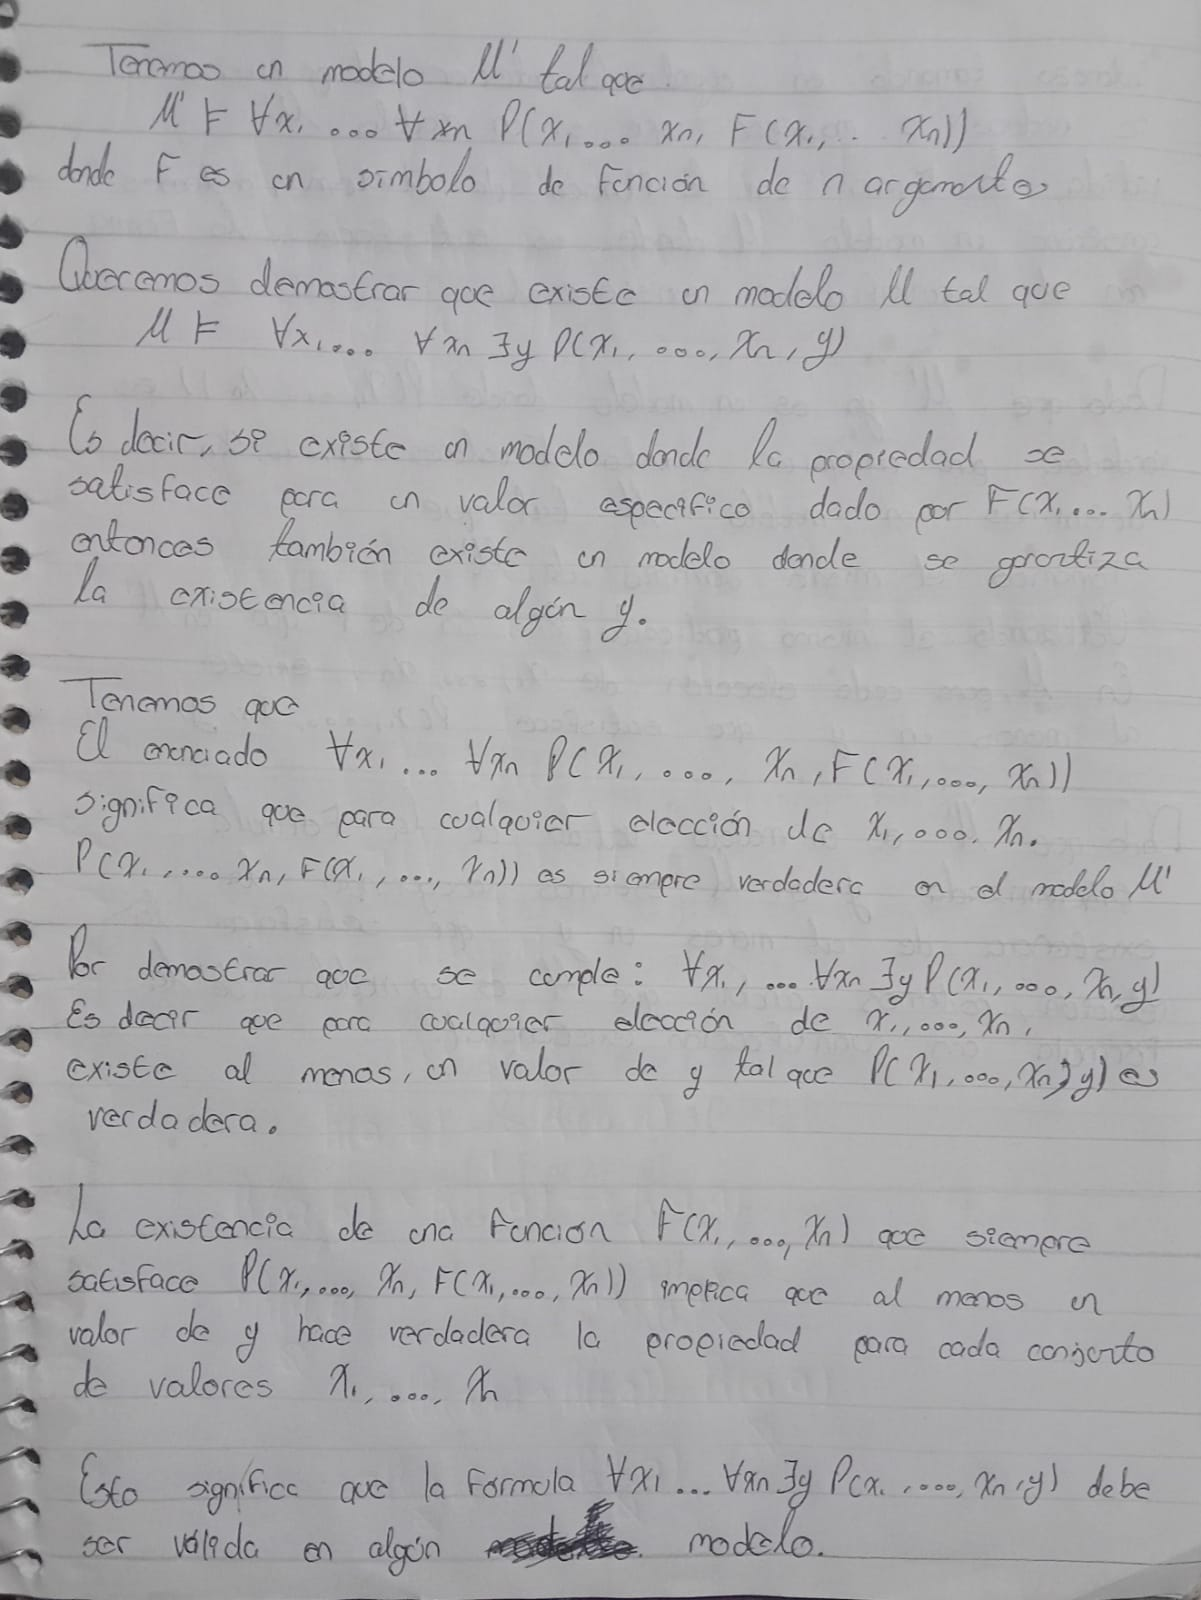
\includegraphics[width=\textwidth,height=0.8\textheight,keepaspectratio]{ejercicio3a.png}
  \end{center}

  \newpage
  
  \begin{center}
    \hspace{-1.2cm} 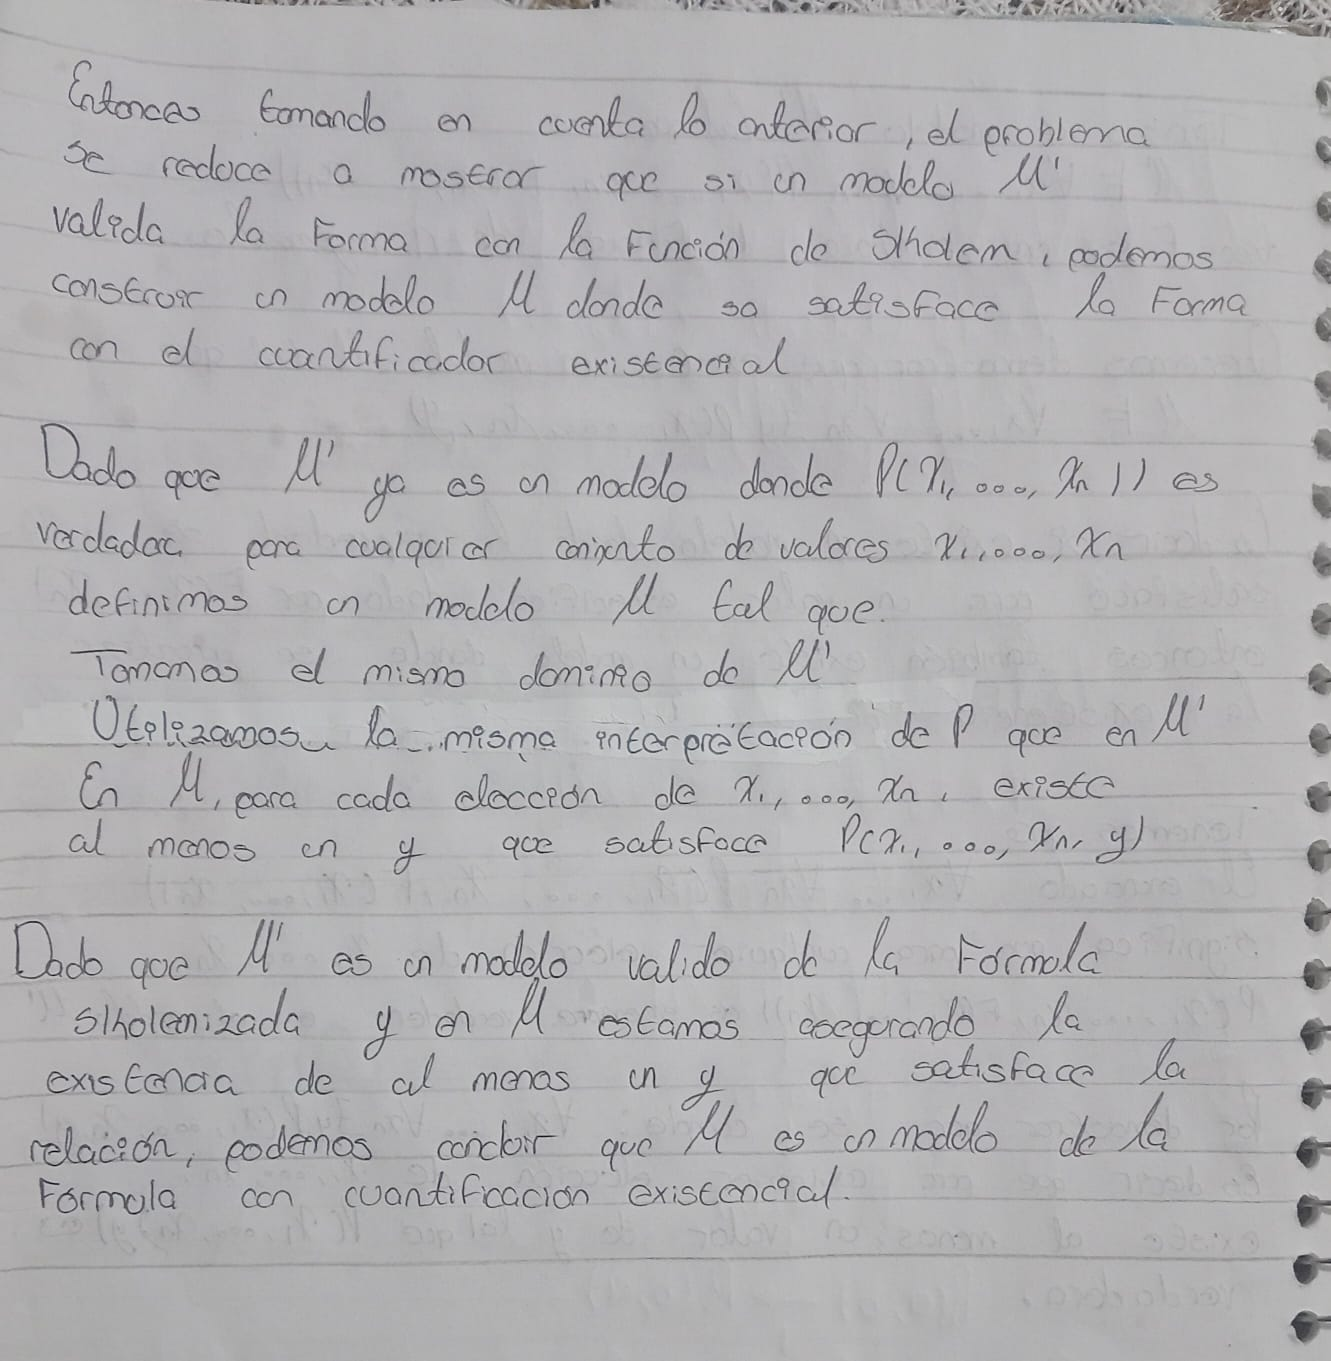
\includegraphics[width=\textwidth,height=0.8\textheight,keepaspectratio]{ejercicio3b.png}
  \end{center}

  \newpage
  
\item (1.5 pts.) Ejecute el algoritmo de Martelli y Montanari sobre las siguientes ecuaciones de términos. En cada caso muestre el unificador más general o la razón por la cual los términos no pueden ser unificados.
  \[
  x = f(a), \quad \quad \quad \quad b = b,
  \]
  \[
  g(f(a)) = y, \quad \quad \quad \quad x = g(y),
  \]
  \[
  \quad \quad \; f(x) = y. \quad \quad \quad \quad x = g(g(z)),
  \]
  \[
  \quad \quad \quad \quad \quad \quad \quad \quad \quad y = g(a).
  \]
  % -- Respuesta --
  \bigskip

  Aplicamos el Algoritmo de Martelli y Monatanari para encontrar el posble umg:\\

  \textbf{Input:}
  \[
  x = f(a),
  \]
  \[
  g(f(a)) = y,
  \]
  \[
  f(x) = y.
  \]
  
  \begin{enumerate}[label=\arabic*)]
  \item Transformamos \( t = x \), donde \( t \) no sea una variable, en \( x = t \):
    \[
    x = f(a),
    \]
    \[
    y = g(f(a)),
    \]
    \[
    y = f(x).
    \]
  
  \item \checkmark No se necesita aplicar la regla dos:
    \[
    x = f(a),
    \]
    \[
    y = g(f(a)),
    \]
    \[
    y = f(x).
    \]

  \item \checkmark No es necesario aplicar la regla tres:
    \[
    x = f(a),
    \]
    \[
    y = g(f(a)),
    \]
    \[
    y = f(x).
    \]

  \item Reemplazamos todas las presencias de $x$ por $f(a)$ en las dem\'{a}s ecuaciones donde $x$ figura.
    \[
    x = f(a),
    \]
    \[
    y = g(f(a)),
    \]
    \[
    y = f(f(a)).
    \]
  \end{enumerate}
  
  Notemos que tenemos $y = g(f(a)),\; y = f(f(a))$, entonces podemos decir que\\
  $g(f(a)) = f(f(a))$, una ecuaci\'{o}n donde ambos lado de la igualdad no son varibales.

  Por la regla 3. \textit{Si el s\'{i}mbolo de funci\'{o}n m\'{a}s externo de t y s no es el mismo, el algoritmo termina reportando no unificable.}. Para este caso $t = g(f(a)),\; s = f(f(a))$, de modo que el conjunto de ecuaciones de t\'{e}rminos dado no se le puede asignar un unificador.
  
  \begin{center}
    \textbf{Output:} \textit{No unificable}
  \end{center}
 
  \textbf{Input:}
  \[
  b = b,
  \]
  \[
  x = g(y),
  \]
  \[
  x = g(g(z)),
  \]
  \[
  y = g(a).
  \]
  
  \begin{enumerate}[label=\arabic*)]
  \item \checkmark No se necesita aplicar la regla uno:
    \[
    b = b,
    \]
    \[
    x = g(y),
    \]
    \[
    x = g(g(z)),
    \]
    \[
    y = g(a).
    \]
    
  \item Eliminamos la ecuaciones de la forma \( x = x \), por lo que quitamos \( b = b \):
    \[
    x = g(y),
    \]
    \[
    x = g(g(z)),
    \]
    \[
    y = g(a).
    \]
  \end{enumerate}

  \begin{enumerate}[label=\arabic*), start=4]
  \item Reemplazamos todas las presencias de $y$ por $g(a)$ en las dem\'{a}s ecuaciones donde $y$ figura:
    \[
    x = g(g(a)),
    \]
    \[
    x = g(g(z)),
    \]
    \[
    y = g(a).
    \]
  \end{enumerate}

  \begin{enumerate}[label=\arabic*), start=3]
  \item Notemos que podemos aplicar la regla 3 a las ecuaciones $x = g(g(a))$, $x = g(g(z))$:
    \[
    x = g(g(a)),
    \]
    \[
    x = g(g(z)),
    \]
    \[
    g(g(a)) = g(g(z)),
    \]
    \[
    g(a) = g(z),
    \]
    \[
    a = z,
    \]
    \[
    y = g(a).
    \]

    Por lo que al simplemente tenemos:
    \[
    x = g(g(a)),
    \]
    \[
    x = g(g(z)),
    \]
    \[
    a = z,
    \]
    \[
    y = g(a).
    \]

  \item Reemplazamos todas las presencias de $a$ por $z$ en las dem\'{a}s ecuaciones donde $a$ figura:
    \[
    x = g(g(z)),
    \]
    \[
    x = g(g(z)),
    \]
    \[
    a = z,
    \]
    \[
    y = g(z).
    \]

    Dado que $x = g(g(z))$ se repite, podemos simplificar y tenemos:
    \[
    x = g(g(z)),
    \]
    \[
    a = z,
    \]
    \[
    y = g(z).
    \]
  \end{enumerate}

  As\'{i} terminamos exitosamente el algoritmo, y afirmamos que:
  \begin{center}
    \textbf{Output:} $\mu = [x := g(g(z)),\; a := z,\; y := g(z)]$
  \end{center}

  Comprobamos aplicando el umg:
  \[
  b = b, \quad \Rightarrow \quad b = b,
  \]
  \[
  x = g(y), \quad \Rightarrow \quad g(g(z)) = g(g(z)),
  \]
  \[
  x = g(g(z)), \quad \Rightarrow \quad g(g(z)) = g(g(z)),
  \]
  \[
  y = g(a). \quad \Rightarrow \quad g(z) = g(z).
  \]
  
  Podemos verificar tambi\'{e}n que el unificador:
  \[
  \theta = [x := g(g(h(b))),\; a := h(b),\; y := g(h(b)),\; z := h(b)]
  \]
  puede expresarse como $\theta = \mu[z := h(b)]$
  
  \newpage
  
\item (1.5 pts.) Unifique los siguientes pares de fórmulas atómicas, si es posible. En caso afirmativo, emplee el algoritmo de Robinson. En caso contrario, dé la razón por la que no pueden ser unificados.

  \begin{center}
      \ding{70} \( Q(g(a,x), g(u,b)), \; Q(z, g(u,x)). \) \quad \quad
      \ding{70} \( P(x, g(z), g(z)), \; P(h(y), y, g(h(x))). \)
  \end{center}
  
  % -- Respuesta --
  \begin{center}
    \hspace{-1.2cm} 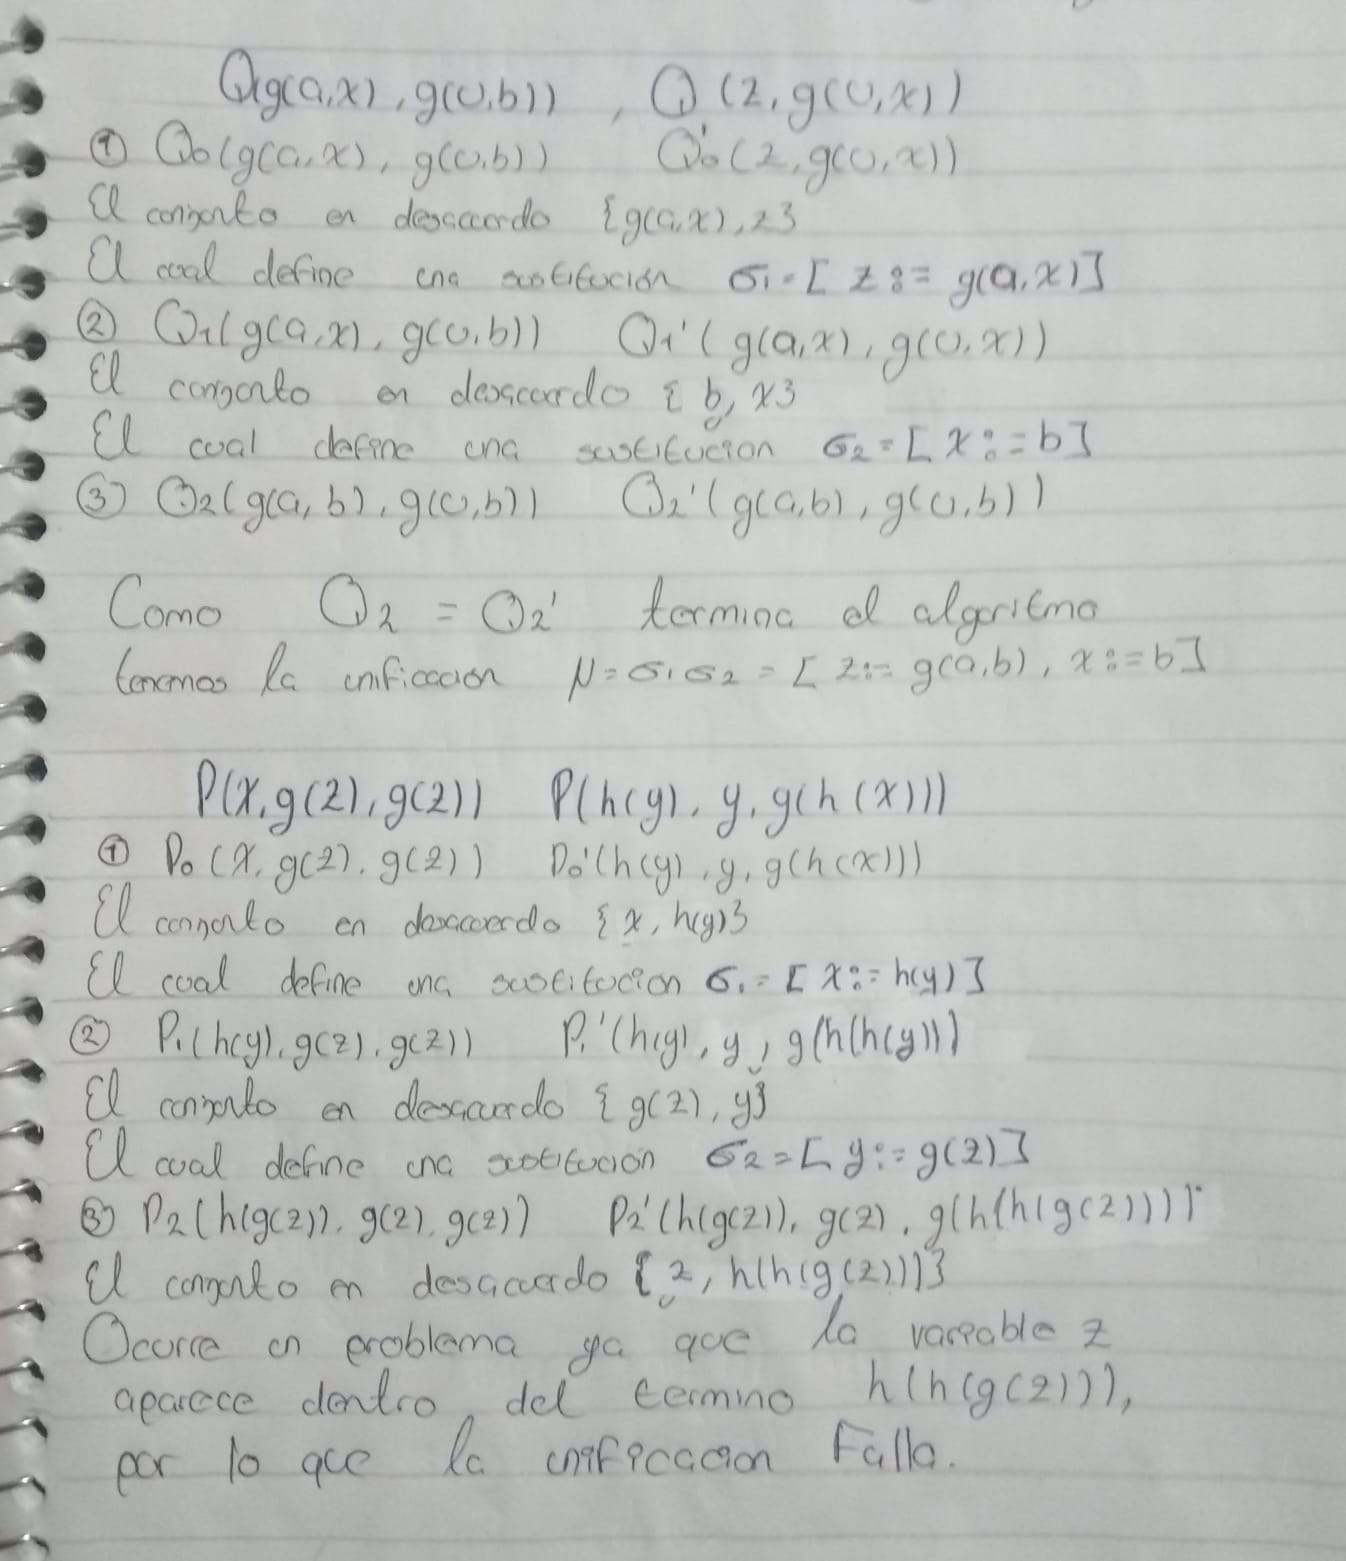
\includegraphics[width=\textwidth,height=0.9\textheight,keepaspectratio]{ejercicio5.png}
  \end{center}
  
\item (1 pt.) ¿Qué es lo que sucede al tratar de unificar las siguientes ecuaciones de términos:  
  \[
  x = f(y), \quad y = g(x)?
  \]
  % -- Respuesta --
  \begin{center}
    \hspace{-1.2cm} 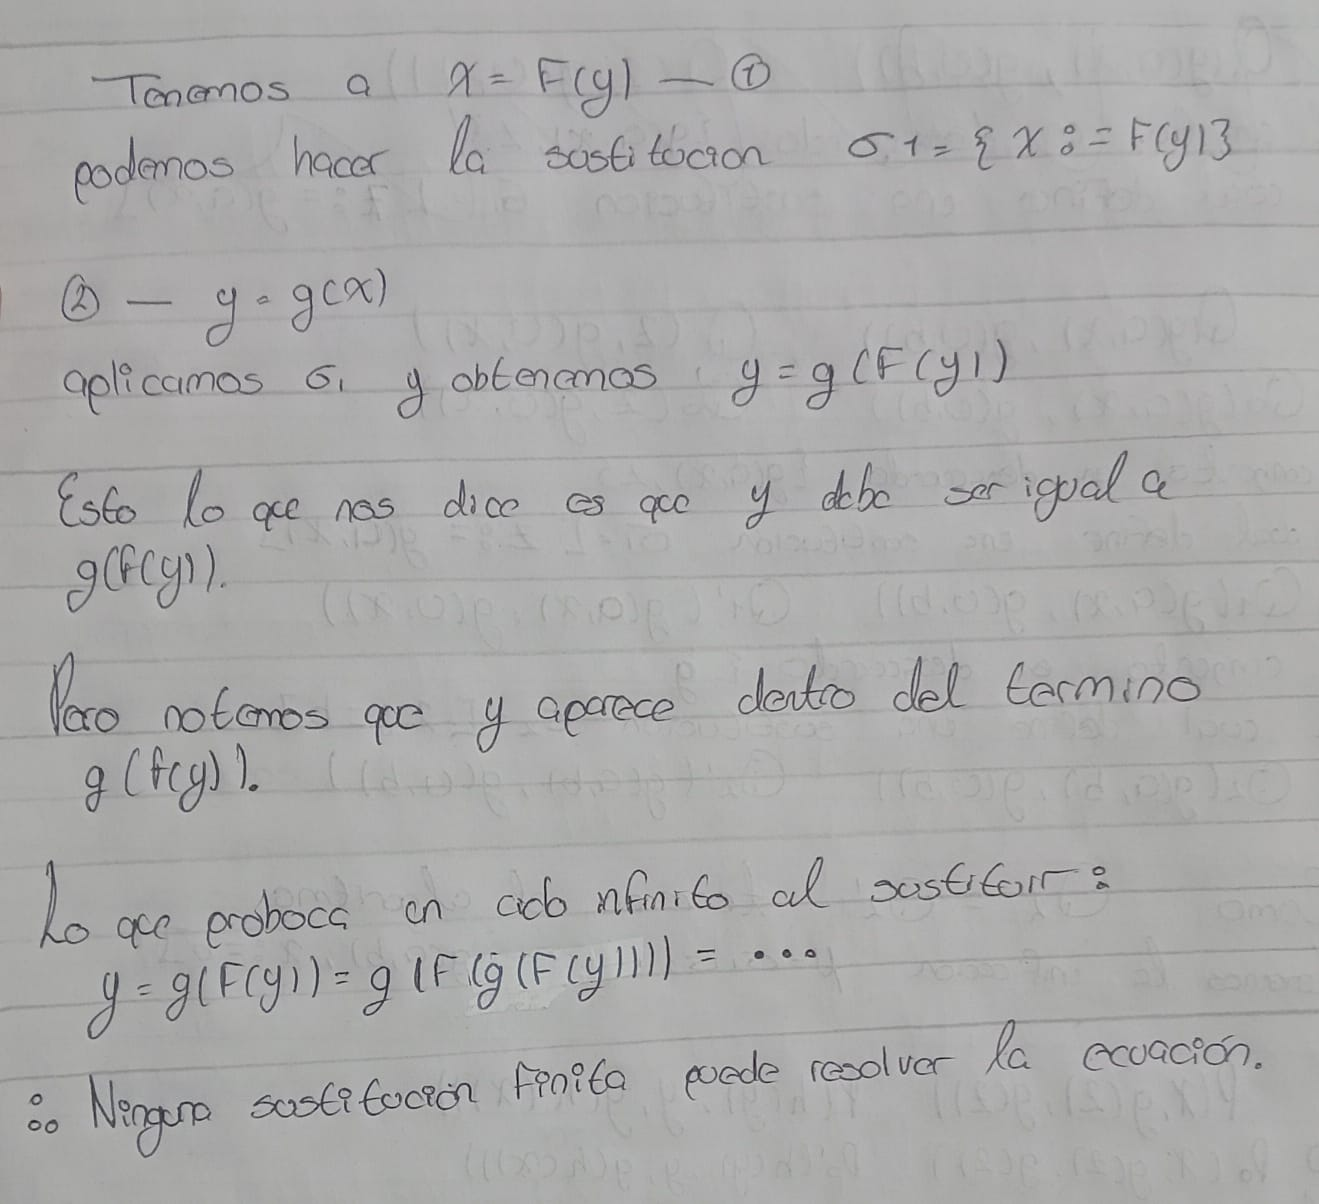
\includegraphics[width=\textwidth,height=0.9\textheight,keepaspectratio]{ejercicio6.png}
  \end{center}

  \newpage
  
\item (2 pts.) Dado \(\forall x \forall y \forall z (P(x,y) \lor P(y,z) \imp P(x,z)), \; \forall x P(x,a), \; \text{y} \; \forall y P(a,y)\),\\
  use resolución para demostrar \( \forall x \forall y P(x,y) \).
  % -- Respuesta --
  \bigskip

  Convertimos cada f\'{o}rmula en su forma normal clausular:

  \begin{itemize}
  \item \( \forall x \forall y \forall z \Big(\big(P(x, y) \land P(y, z)\big) \imp P(x, z) \Big) \)
    
    \( \hspace{0.8cm} \Rightarrow \big(P(x, y) \land P(y, z)\big) \imp P(x, z) \equiv \neg \big(P(x, y) \land P(y, z)\big) \lor P(x, z) \)

    \( \hspace{1.5cm} \equiv \neg P(x, y) \lor \neg P(y, z) \lor P(x, z) \)

    \( \hspace{1.86cm} \Rightarrow \{\; {\neg P(x, y),\: \neg P(y, z),\: P(x, z) }\; \} \)

  \item \( \forall x P(x, a) \Rightarrow \{\; P(x, a)\; \} \)
  \item \( \forall y P(a, y) \Rightarrow \{\; P(a, y)\; \} \)
  \item Tenemos el consecuente \( \forall x \forall y P(x, y) \), por lo que lo negamos y tenemos:

    \( \neg \big(\forall x \forall y P(x, y)\big) \equiv \neg \forall x \neg \forall y \neg P(x, y) \equiv \exists x \exists y \neg P(x, y) \)

    Aplicando la \textit{Skolemizaci\'{o}n}, dado que no hay alg\'{u}n cuantificador universal antes de ambos cuantificadores existenciales, entonces los argumentos de $P$ son constantes:
    
    \( \hspace{1.86cm} \Rightarrow \{\; \neg P(b, c)\;  \} \)
  \end{itemize}

  Dado el conjunto $S =$ \( \Big\{\: \{\: \neg P(x, y),\: \neg P(y, z),\: P(x, z) \: \}, \; \{\: P(x, a)\: \},\;  \{\: P(a, y)\: \},\; \{\: \neg P(b, c)\: \} \:\Big\} \)

  Realizamos el Procedimiento de Resoluci\'{o}n General:
  
  \begin{center}
    \begin{enumerate}[label=\arabic*.]
    \item \( \{\; \neg P(x, y),\: \neg P(y, z),\: P(x, z) \; \} \) \quad \textit{Prem}
    \item \( \{\; P(x, a)\; \} \) \hspace{3.9cm} \textit{Prem}
    \item \( \{\; P(a, y)\; \} \) \hspace{3.9cm} \textit{Prem}
    \item \( \{\; \neg P(b, c)\; \} \) \hspace{3.7cm} \textit{Prem}
    \item \( \{\; \neg P(a, z),\; P(x, z)\; \}\) \hspace{0.2cm} $[y := a]$ \hspace{0.22cm} \textit{Res} (1, 2)
    \item \( \{\; P(x, z)\; \}\) \hspace{2.05cm} $[z := y]$ \hspace{0.22cm} \textit{Res} (3, 5)
    \item $\scalebox{1.3}{$\square$}$ \hspace{2.23cm} $[x := b,\; y := c]$ \hspace{0.22cm} \textit{Res} (4, 6)
    \end{enumerate}
  \end{center}

  Llegamos a la cl\'{a}usula vac\'{i}a, $\square$, por lo que el conjunto $S$ es insatisfacible.

  \[
  \therefore \text{ Se cumple } \forall \text{$x$} \forall \text{$y$} \text{$P(x,y)$}
  \]
  
\end{enumerate}

\end{document}
